\subsection{Objetivo 5: Evaluar cualitativamente la precisión y suavidad del sistema de localización}

\textbf{Fase 1: Pruebas de campo}

Las primeras pruebas de campo tuvieron como propósito observar el comportamiento del sistema de localización tanto en reposo como en movimiento, verificando la coherencia visual entre la posición estimada del usuario y la dirección mostrada en la aplicación de realidad aumentada. Inicialmente se efectuó una prueba de concepto en un entorno controlado —una habitación— en la que se dispusieron cuatro sensores UWB (beacons) de Estimote colocados en disposición rectangular. En este entorno se probó la integración completa entre el sistema de multilateración, el filtro de Kalman y la aplicación desarrollada en Unity. % Se enfatiza la conexión completa del sistema en la app final.

Durante las pruebas se observó el mapa desde vista superior para visualizar el posicionamiento del jugador en el entorno virtual y posteriormente se evaluó la flecha de realidad aumentada que indica la dirección del objetivo. En todos los casos, la flecha apuntó de forma consistente hacia el objetivo y los movimientos fueron suaves y estables, confirmando la correcta fusión entre el algoritmo de multilateración y el filtro de Kalman. No se detectaron comportamientos erráticos ni fluctuaciones visuales significativas. % Esta afirmación valida la precisión cualitativa del sistema en condiciones controladas.

\begin{figure}[H]
    \centering
    % Subfigura 1: vista superior
    \begin{subfigure}[b]{0.45\textwidth}
        \centering
        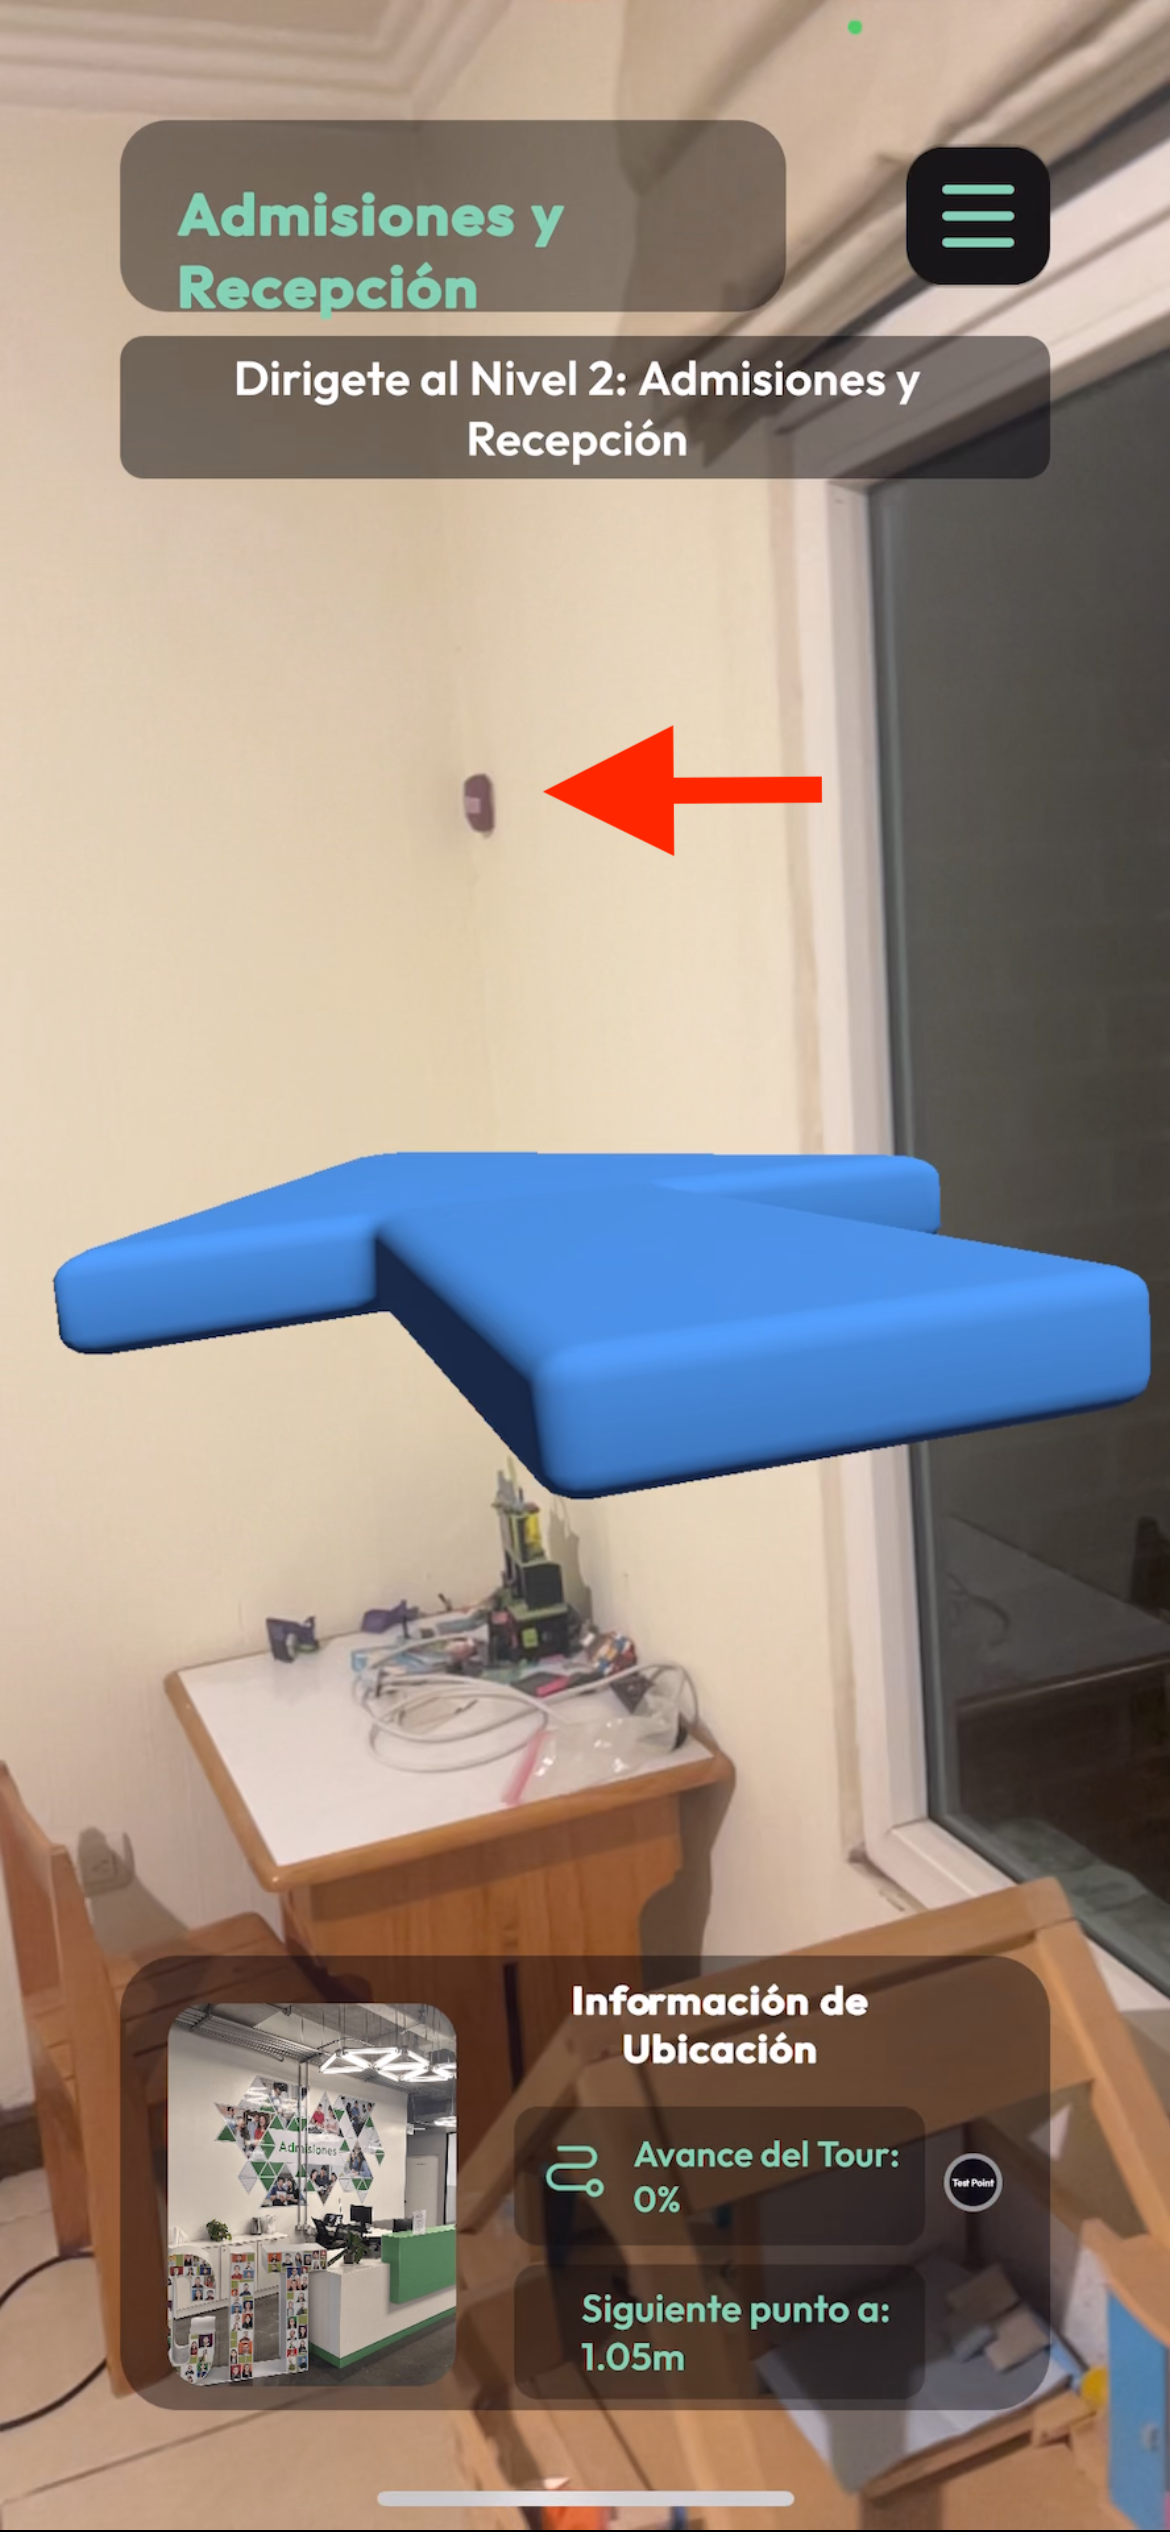
\includegraphics[height=0.45\textheight]{images/pov1.PNG} % ajusta 0.45 si aún se ven grandes
        \caption{Vista de la flecha apuntando al objetivo correctamente (señalado en rojo).}
        \label{fig:home_test_topview}
    \end{subfigure}
    \hfill
    % Subfigura 2: trayectoria general
    \begin{subfigure}[b]{0.45\textwidth}
        \centering
        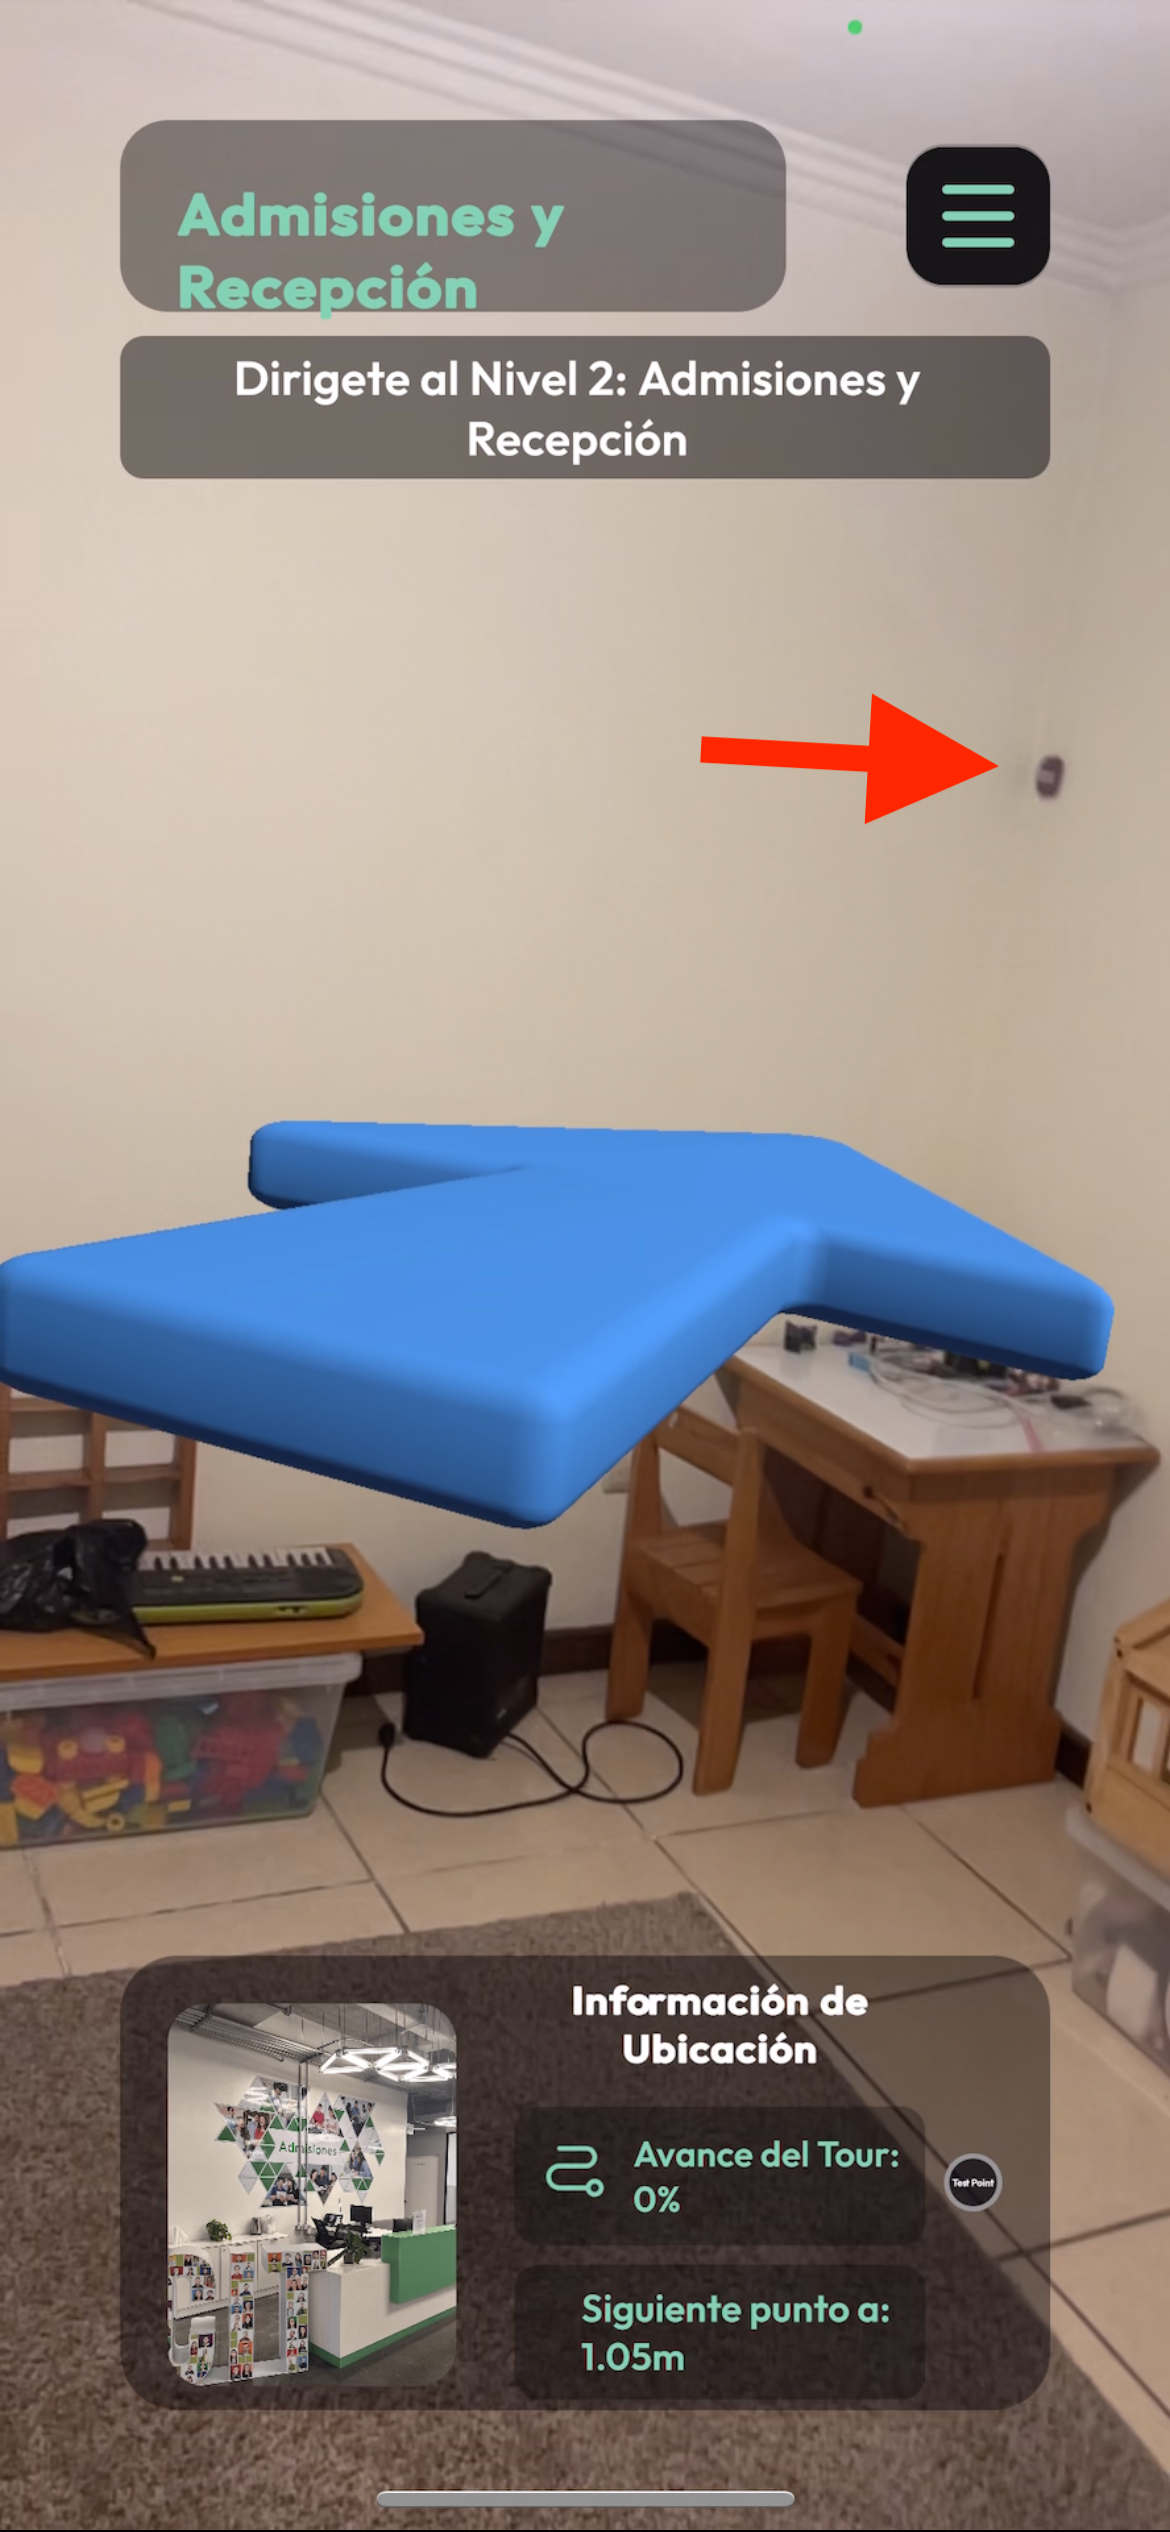
\includegraphics[height=0.45\textheight]{images/pov2.PNG}
        \caption{Vista de la flecha apuntando al objetivo correctamente (señalado en rojo).}
        \label{fig:home_test_path}
    \end{subfigure}
    \caption{Pruebas domésticas con el sistema completamente integrado. Las trayectorias muestran un movimiento continuo y estable, confirmando la correcta sincronización entre el algoritmo de trilateración, el filtro de Kalman y la aplicación de realidad aumentada.}
    \label{fig:home_test_results}
\end{figure}

A partir de estos resultados iniciales, se trasladaron las pruebas al entorno real de la Universidad del Valle de Guatemala, específicamente al sexto nivel del edificio. En esta etapa se utilizaron cinco sensores, distribuidos según las coordenadas obtenidas experimentalmente:

\begin{verbatim}
{
  "44d22f737b259dd4e31a23b324ef941f": { "x": 12.95, "y": 4.49, "z": 2.5 },
  "550aed08145ffba276256b188a968124": { "x": 16.99, "y": -2.89, "z": 2.5 },
  "420139767c96fee20dec018c2ec7a33a": { "x": 19.26, "y": 4.99, "z": 2.5 },
  "dc89a1ea448ecf9b5c8f9f66af1ecc06": { "x": 13.03, "y": 12.2, "z": 2.5 },
  "fe08fa755807f79abf1a233724ed182e": { "x": 14.58, "y": 22.94, "z": 2.5 }
}
\end{verbatim}

Los sensores se encontraban instalados a una altura de aproximadamente 2.5 metros, separados entre 10 y 15 metros. Durante esta etapa se observaron múltiples dificultades en la conectividad con los sensores, ya que el dispositivo móvil raramente lograba mantener conexión con más de tres sensores simultáneamente. Además, los tiempos de actualización eran inconsistentes, lo que generaba saltos abruptos en la posición estimada. % Este párrafo describe el contexto experimental real y los problemas empíricos observados.

Estas limitaciones llevaron a plantear tres hipótesis principales: (1) interferencia electromagnética causada por la gran cantidad de señales BLE, Wi-Fi y dispositivos electrónicos en el campus; (2) desgaste en las baterías de los sensores, adquiridos un año antes; y (3) exceso de separación y altura de instalación, lo que reducía la calidad de la señal recibida por el dispositivo móvil. % Se explican las causas técnicas y su justificación.


\textbf{Fase 2: Recolección y análisis de datos}

Con el fin de analizar la estabilidad visual y la suavidad de movimiento, se registraron observaciones cualitativas del sistema en funcionamiento. En las pruebas realizadas en el entorno doméstico, la estabilidad visual fue óptima, por lo que no se requirieron modificaciones adicionales ni al filtro de Kalman ni al algoritmo de multilateración. % Se destaca que el sistema base funcionó correctamente en condiciones controladas.

En contraste, las pruebas en el entorno universitario presentaron un movimiento inconsistente. En varios casos el marcador virtual permanecía estable durante algunos segundos, pero luego sufría desplazamientos erráticos o retrasos notables en la actualización de posición. Este comportamiento se atribuyó a la falta de sincronización en las actualizaciones de distancia, ya que en múltiples ocasiones únicamente se recibían datos de uno o dos sensores, impidiendo una trilateración precisa. % Este comentario indica el origen técnico del jitter visual.

Los datos de posicionamiento obtenidos en estas pruebas se emplearán para generar gráficas comparativas que reflejen el jitter y la dispersión espacial del sistema. % Punto sugerido para incluir gráfica.
% ===> Aquí puedes incluir una figura con capturas de pantalla del recorrido en el entorno universitario.
% Ejemplo: 
\begin{figure}[H]
    \centering
    % Subfigura 1: vista superior del mapa
    \begin{subfigure}[b]{0.45\textwidth}
        \centering
        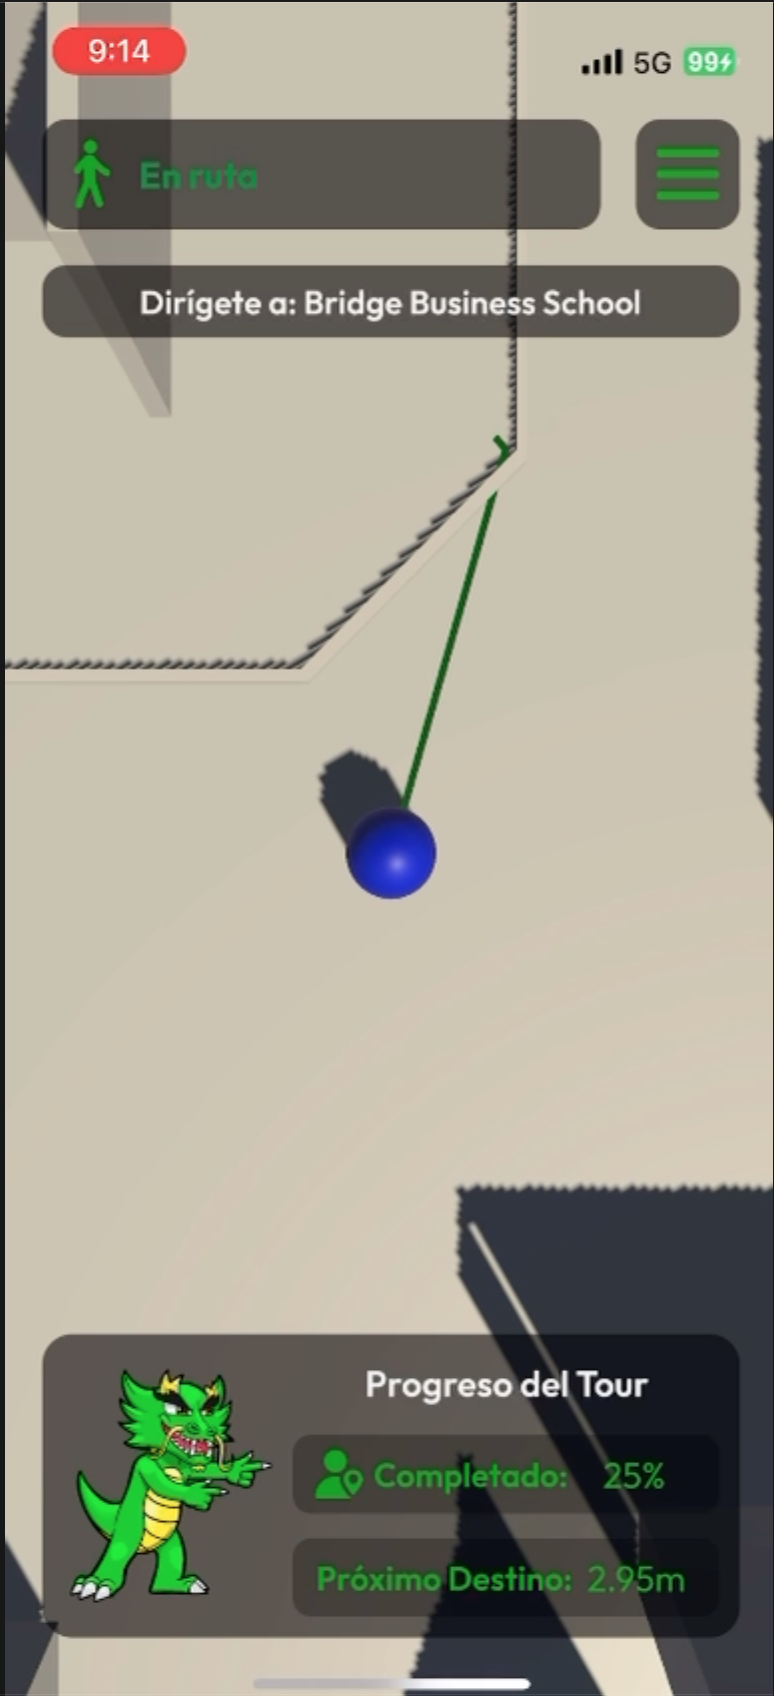
\includegraphics[height=0.38\textheight]{images/unity_route.png}
        \caption{Vista superior del mapa con la trayectoria del usuario en el entorno universitario.}
        \label{fig:unity_map_view}
    \end{subfigure}
    \hfill
    % Subfigura 2: vista en primera persona (AR)
    \begin{subfigure}[b]{0.45\textwidth}
        \centering
        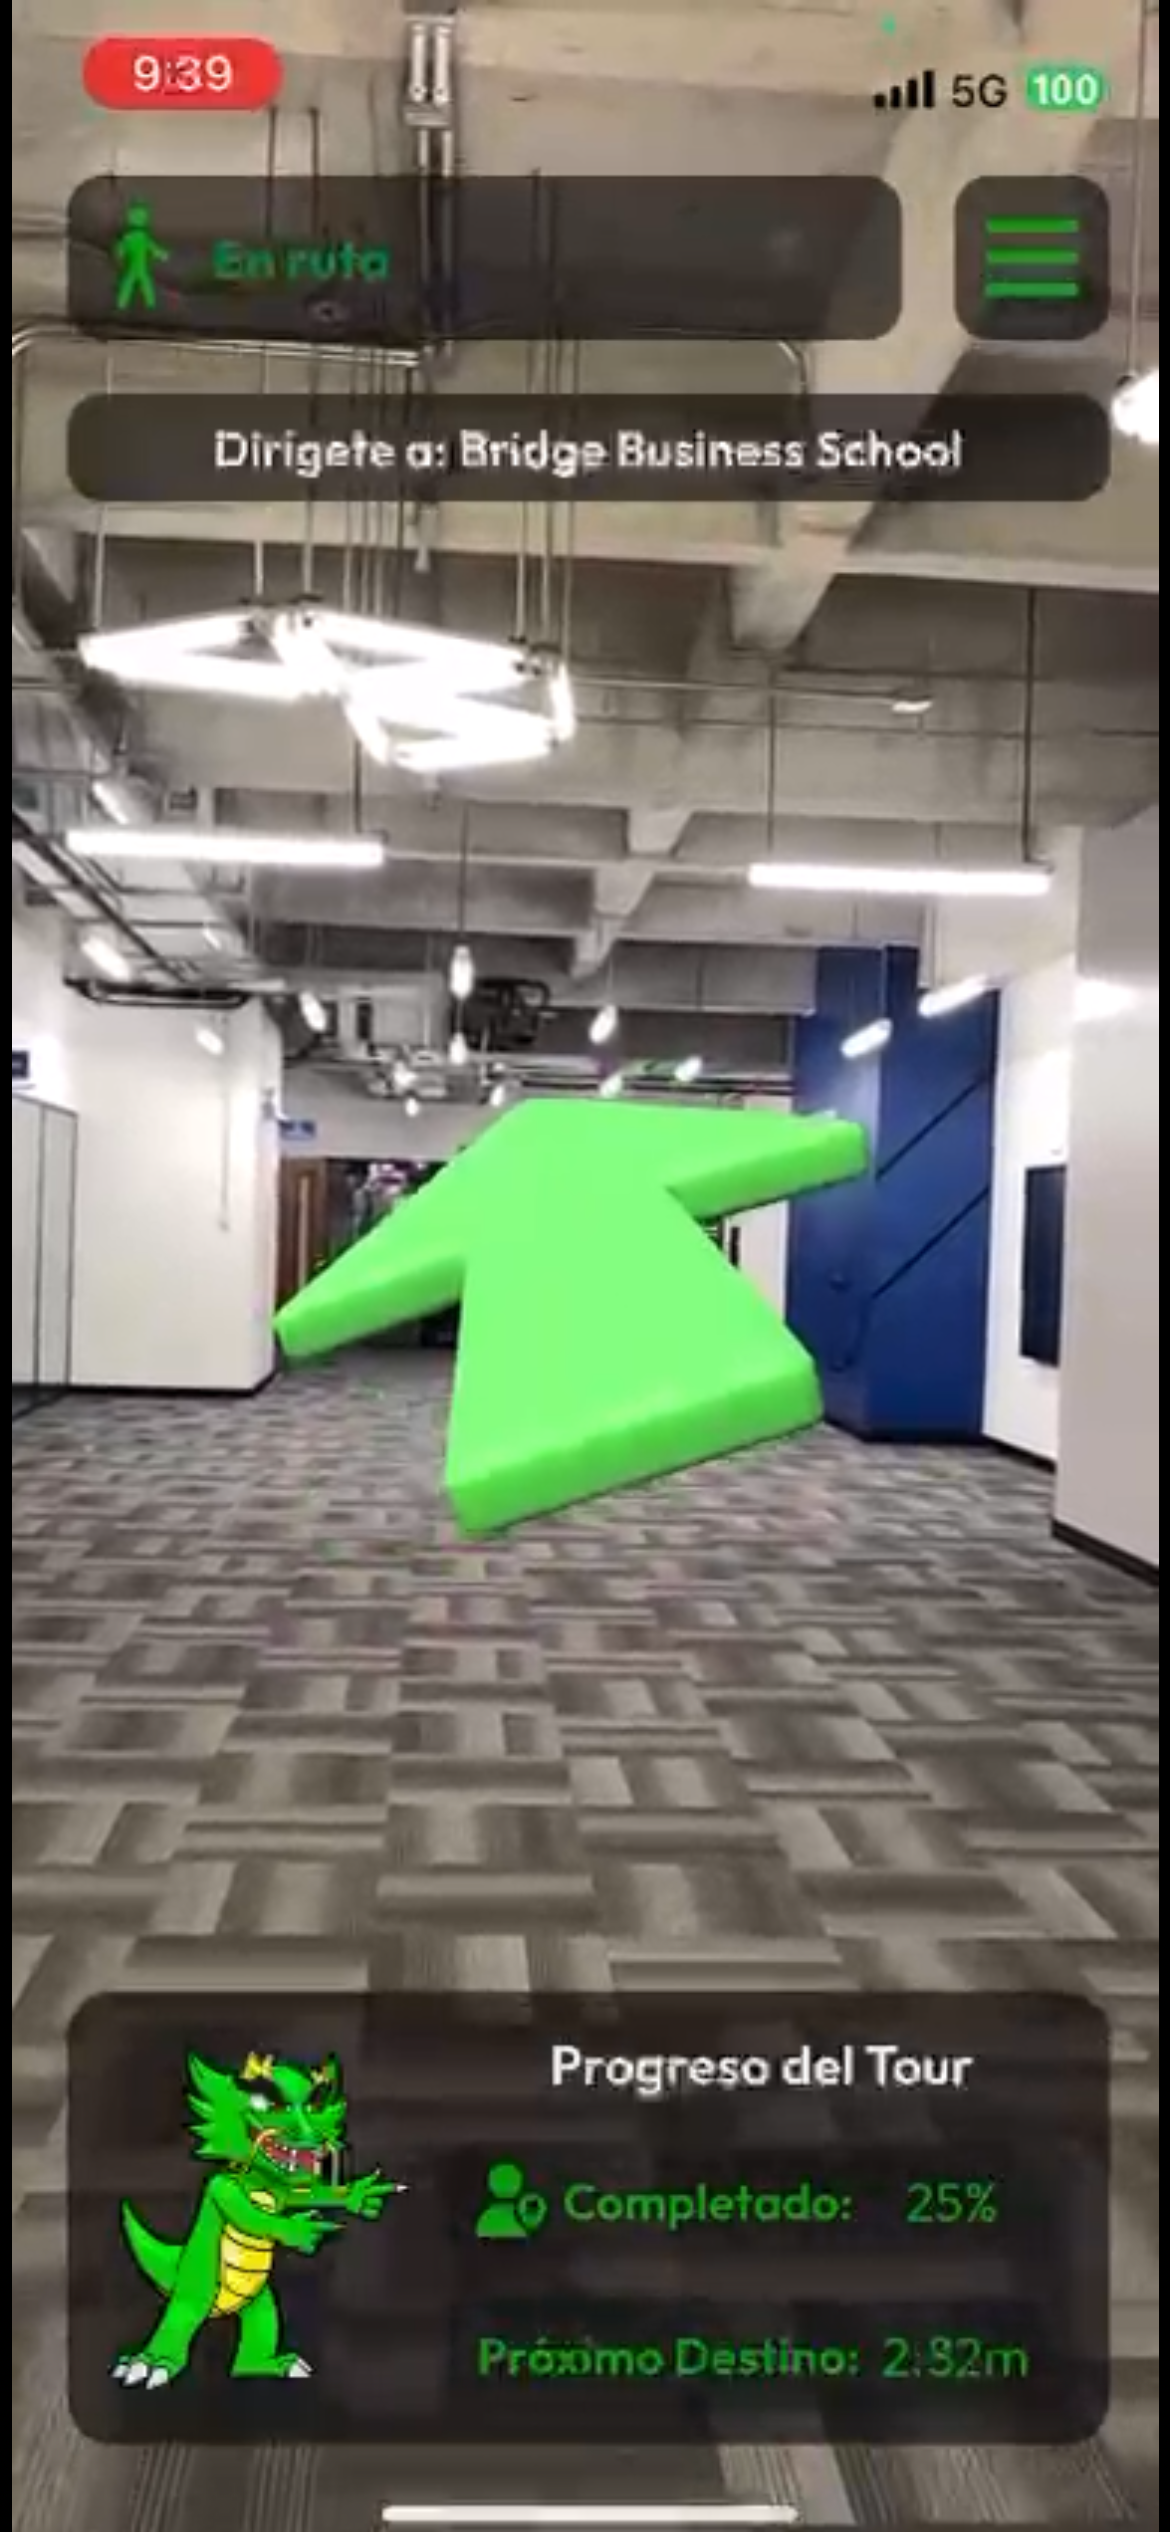
\includegraphics[height=0.38\textheight]{images/pov3.PNG}
        \caption{Vista en primera persona desde la aplicación de realidad aumentada, mostrando la flecha direccional hacia el objetivo.}
        \label{fig:unity_firstperson_view}
    \end{subfigure}
    \caption{Pruebas en el entorno universitario mostrando la trayectoria del usuario (izquierda) y la visualización en realidad aumentada (derecha). Ambas perspectivas confirman la coherencia entre la posición estimada y la dirección mostrada al usuario.}
    \label{fig:unity_combined_views}
\end{figure}

Asimismo, se incluirán capturas de pantalla representativas del comportamiento visual del sistema durante las pruebas, con el fin de complementar el análisis cualitativo. % Punto sugerido para incluir capturas de la aplicación.


\textbf{Fase 3: Ajustes iterativos}

Como parte del proceso de mejora, se procedió a reemplazar las baterías de los sensores, reducir la distancia entre ellos y disminuir la altura de instalación a aproximadamente 1.65 metros. Estas modificaciones mejoraron parcialmente la estabilidad de la conexión, lo que permitió continuar con nuevas pruebas. % Se describe la iteración física sobre la configuración de sensores.

Adicionalmente, se identificó una limitación técnica importante en el \textit{Software Development Kit} (SDK) de Estimote, utilizado para gestionar las conexiones con los sensores desde la aplicación desarrollada en Swift e integrada posteriormente con Unity. Inicialmente, el sistema mantenía un límite de seis conexiones simultáneas, suficiente para realizar trilateración con redundancia; sin embargo, esto impedía conectar sensores adyacentes y obstaculizaba la continuidad del recorrido. % Se introduce el origen del problema en la capa de comunicación.

Para mitigar esta restricción, el límite de conexiones se aumentó a 100, lo cual generó un nuevo error interno de calendarización de hilos (\textit{EXC BAD ACCESS}). Dicho error provenía directamente del ensamblado del SDK propietario, impidiendo su depuración o modificación. Aunque se intentó realizar un \textit{rollback} a versiones anteriores del plugin, e incluso se probó el SDK de forma aislada, el error persistía al conectar más de seis sensores. % Este comentario explica la imposibilidad de depuración por software propietario.

Es importante destacar que este fallo no se encontraba en la implementación del algoritmo de trilateración ni en el filtro de Kalman, sino en la capa de comunicación proporcionada por el SDK. % Se enfatiza responsabilidad técnica y se protege la validez del modelo matemático.

El SDK de Estimote, al ser software propietario distribuido como binario compilado para Swift, no expone su código fuente ni símbolos de depuración. Esto impide acceder a los procesos internos de manejo de hilos, colas de actualización o temporizadores, limitando la posibilidad de identificar el origen exacto del error o aplicar correcciones a nivel de código. Incluso la aplicación oficial de Estimote presentaba fallas similares al intentar gestionar múltiples conexiones simultáneas, lo cual refuerza la hipótesis de que se trata de una deficiencia estructural del SDK. % Comentario: esta explicación técnica justifica la imposibilidad de solución directa.

Finalmente, el sistema logró mantener un comportamiento estable en entornos controlados, confirmando la efectividad del modelo de filtrado y posicionamiento. No obstante, las limitaciones técnicas del SDK imposibilitaron una evaluación más amplia en entornos reales. % Conclusión de la fase 3.

% ===> Aquí puedes incluir una figura de diagnóstico o esquema de flujo del sistema mostrando el punto donde ocurre el error del SDK.
% Ejemplo: 
\begin{figure}[h] 
  \centering 
  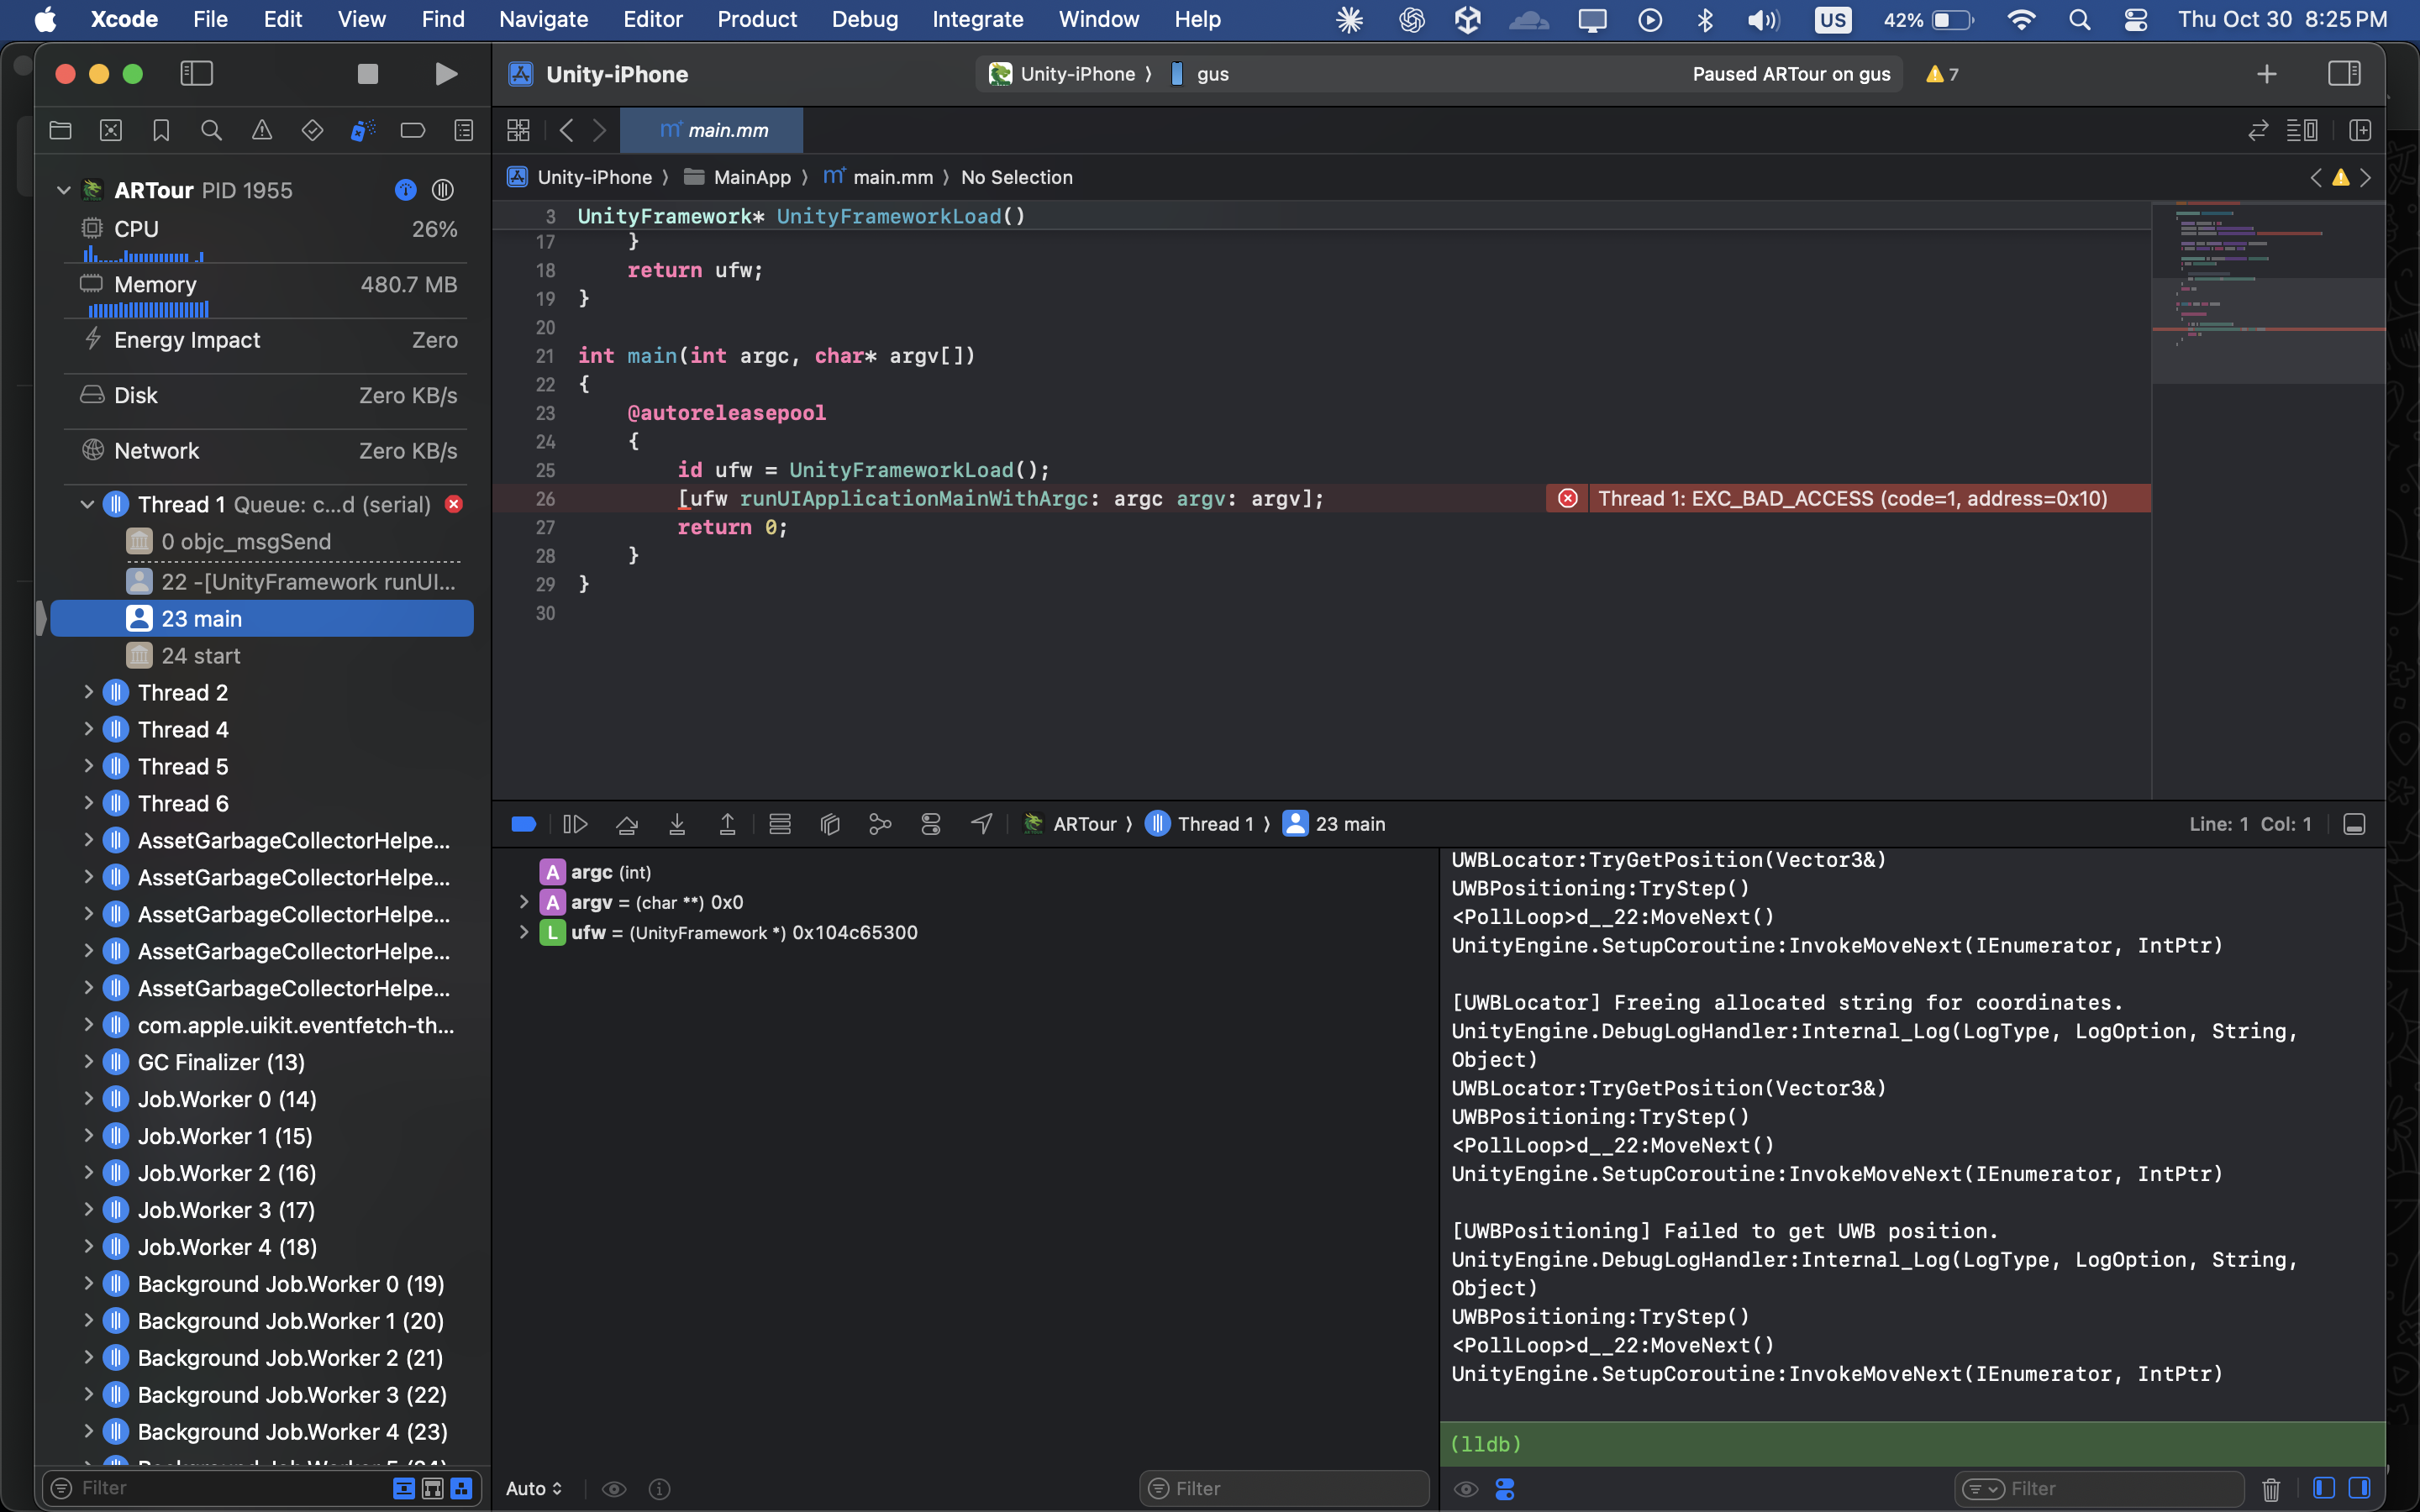
\includegraphics[width=0.6\textwidth]{images/bad_access_error.png} 
  \caption{Log de comunicación entre la aplicación y el SDK de Estimote, donde se origina el error de calendarización.} 
\end{figure}

En síntesis, la evaluación cualitativa del sistema permitió confirmar que el algoritmo de trilateración y el filtro de Kalman operan correctamente en condiciones estables, pero que la capa de comunicación —dependiente de software propietario cerrado— representa la principal limitante para la escalabilidad y confiabilidad del sistema en entornos complejos.